\section{Implementation}

In this section outlines the implementation of the beer information retrieval system, focusing on the key components and technologies used to its development.

The system is composed of two main components: the backend and the frontend. In the following subsections both components will be described in detail to provide a better understanding of the inner workings of the search engine.

\subsection{Backend}

The backend is the core of the entire information retrieval system as it is responsible for the business logic. It offers two main functions: dataset indexing leveraging \textit{PyTerrier}, and two of \textit{REST APIs} to query the index and retrieve the results in JSON format and to perform relevance feedback.

It has been built using \textit{Python} and \textit{FastAPI}, a modern, fast (high-performance), web framework for building APIs. This particular framework has been chosen as it is easy to use, is well documented and allows building APIs in a matter of minutes.

\subsubsection{Endpoints}

As already cited in the previous section, the backend offers two endpoints to interact with the index. Both endpoints are \textit{REST APIs} and are described in detail in the following list:

\begin{enumerate}
  \item \texttt{/search} is the endpoint used to perform a query to the index. It accepts a \texttt{GET} request with the following query parameters:

        \begin{itemize}
          \item \texttt{query}: the query to be performed to the index.
          \item \texttt{top}: the number of results to be returned.
        \end{itemize}

        Example of a request to the \texttt{/search} endpoint:

        \begin{lstlisting}[language=bash]
      curl -X 'GET' \
        'http://localhost:8000/search?query=ipa&top=10' \
        -H 'accept: application/json'
    \end{lstlisting}

  \item \texttt{/feedback} is the endpoint used to perform relevance feedback. It accepts a \texttt{POST} request with the following body parameters:

        \begin{itemize}
          \item \texttt{query}: the query to be performed to the index.
          \item \texttt{relevant}: the list of document IDs that the user considers relevant.
          \item \texttt{irrelevant}: the list of document IDs that the user considers irrelevant.
        \end{itemize}

        Additionally, the \texttt{top} query parameter can be specified to control the number of results to be returned.

        Example of a request to the \texttt{/feedback} endpoint:

        \begin{lstlisting}[language=bash]
        curl -X 'POST' \
          'http://localhost:8000/feedback?top=10' \
          -H 'accept: application/json' \
          -H 'Content-Type: application/json' \
          -d '{
            "query": "ipa",
            "relevant": [
              "d1",
              "d2"
            ],
            "irrelevant": [
              "d3",
              "d4"
            ]
          }'
        \end{lstlisting}
\end{enumerate}

\textit{FastAPI} automatically generates the documentation of the endpoints, which can be accessed at \texttt{http://localhost:8000/docs}. From this page it is possible to interact with the endpoints and test them in real-time directly from the browser.

\subsubsection{Commands}

To simplify the execution of the backend, a \textit{Makefile} is provided to allow the user to easily build the index and start the REST API server. The following commands are available:

\begin{itemize}
  \item \texttt{make build-index} builds the reverse index from the dataset crawled from the web (refer to Section \ref{sec:data-scraping} for more details).
  \item \texttt{make dev} starts the backend in development mode, which means that the server will automatically restart when a change in the code is detected.
  \item \texttt{make start} starts the backend in production mode.
\end{itemize}

\subsection{Frontend}

The frontend, designed carefully to provide a good user experience across all devices, is the component that enable users to interact with the search engine. It is a web application that allows users to perform a search and visualize the results of the query in a user-friendly way. Additionally, it allows users to perform relevance feedback to improve the results of the query.

The \textit{webapp} has been built using advanced web technologies to provide a modern and fast application that respect modern web standards. The following technologies have been used to build the frontend:

\begin{itemize}
  \item \textit{TypeScript} is a programming language developed by Microsoft. It is a superset of JavaScript that adds static typing to the language. It is a very powerful language that allows to build complex web applications.

  \item \textit{NextJS} is a framework built on top of \textit{React.js} that allows to build server-side rendered web applications. It is a very powerful framework that allows to build web applications in a matter of minutes.

  \item \textit{React.js} is a JavaScript library for building user interfaces. It is a very popular library that is used by many companies to build their web applications.

  \item \textit{Chakra UI} is a component library that provides a set of accessible and reusable components that can be used to build user interfaces.
\end{itemize}

The frontend is composed of two main pages: a homepage that allows the user to perform an initial search (refer to Figure \ref{fig:home-page}), and a search page that allows the user to visualize, filter and sort the results of the query (refer to Figure \ref{fig:seach-page}). Additionally, this last page allows the user to perform relevance feedback to improve the results of the given query.

% Home page screenshot
\begin{figure}[H]
  \centering
  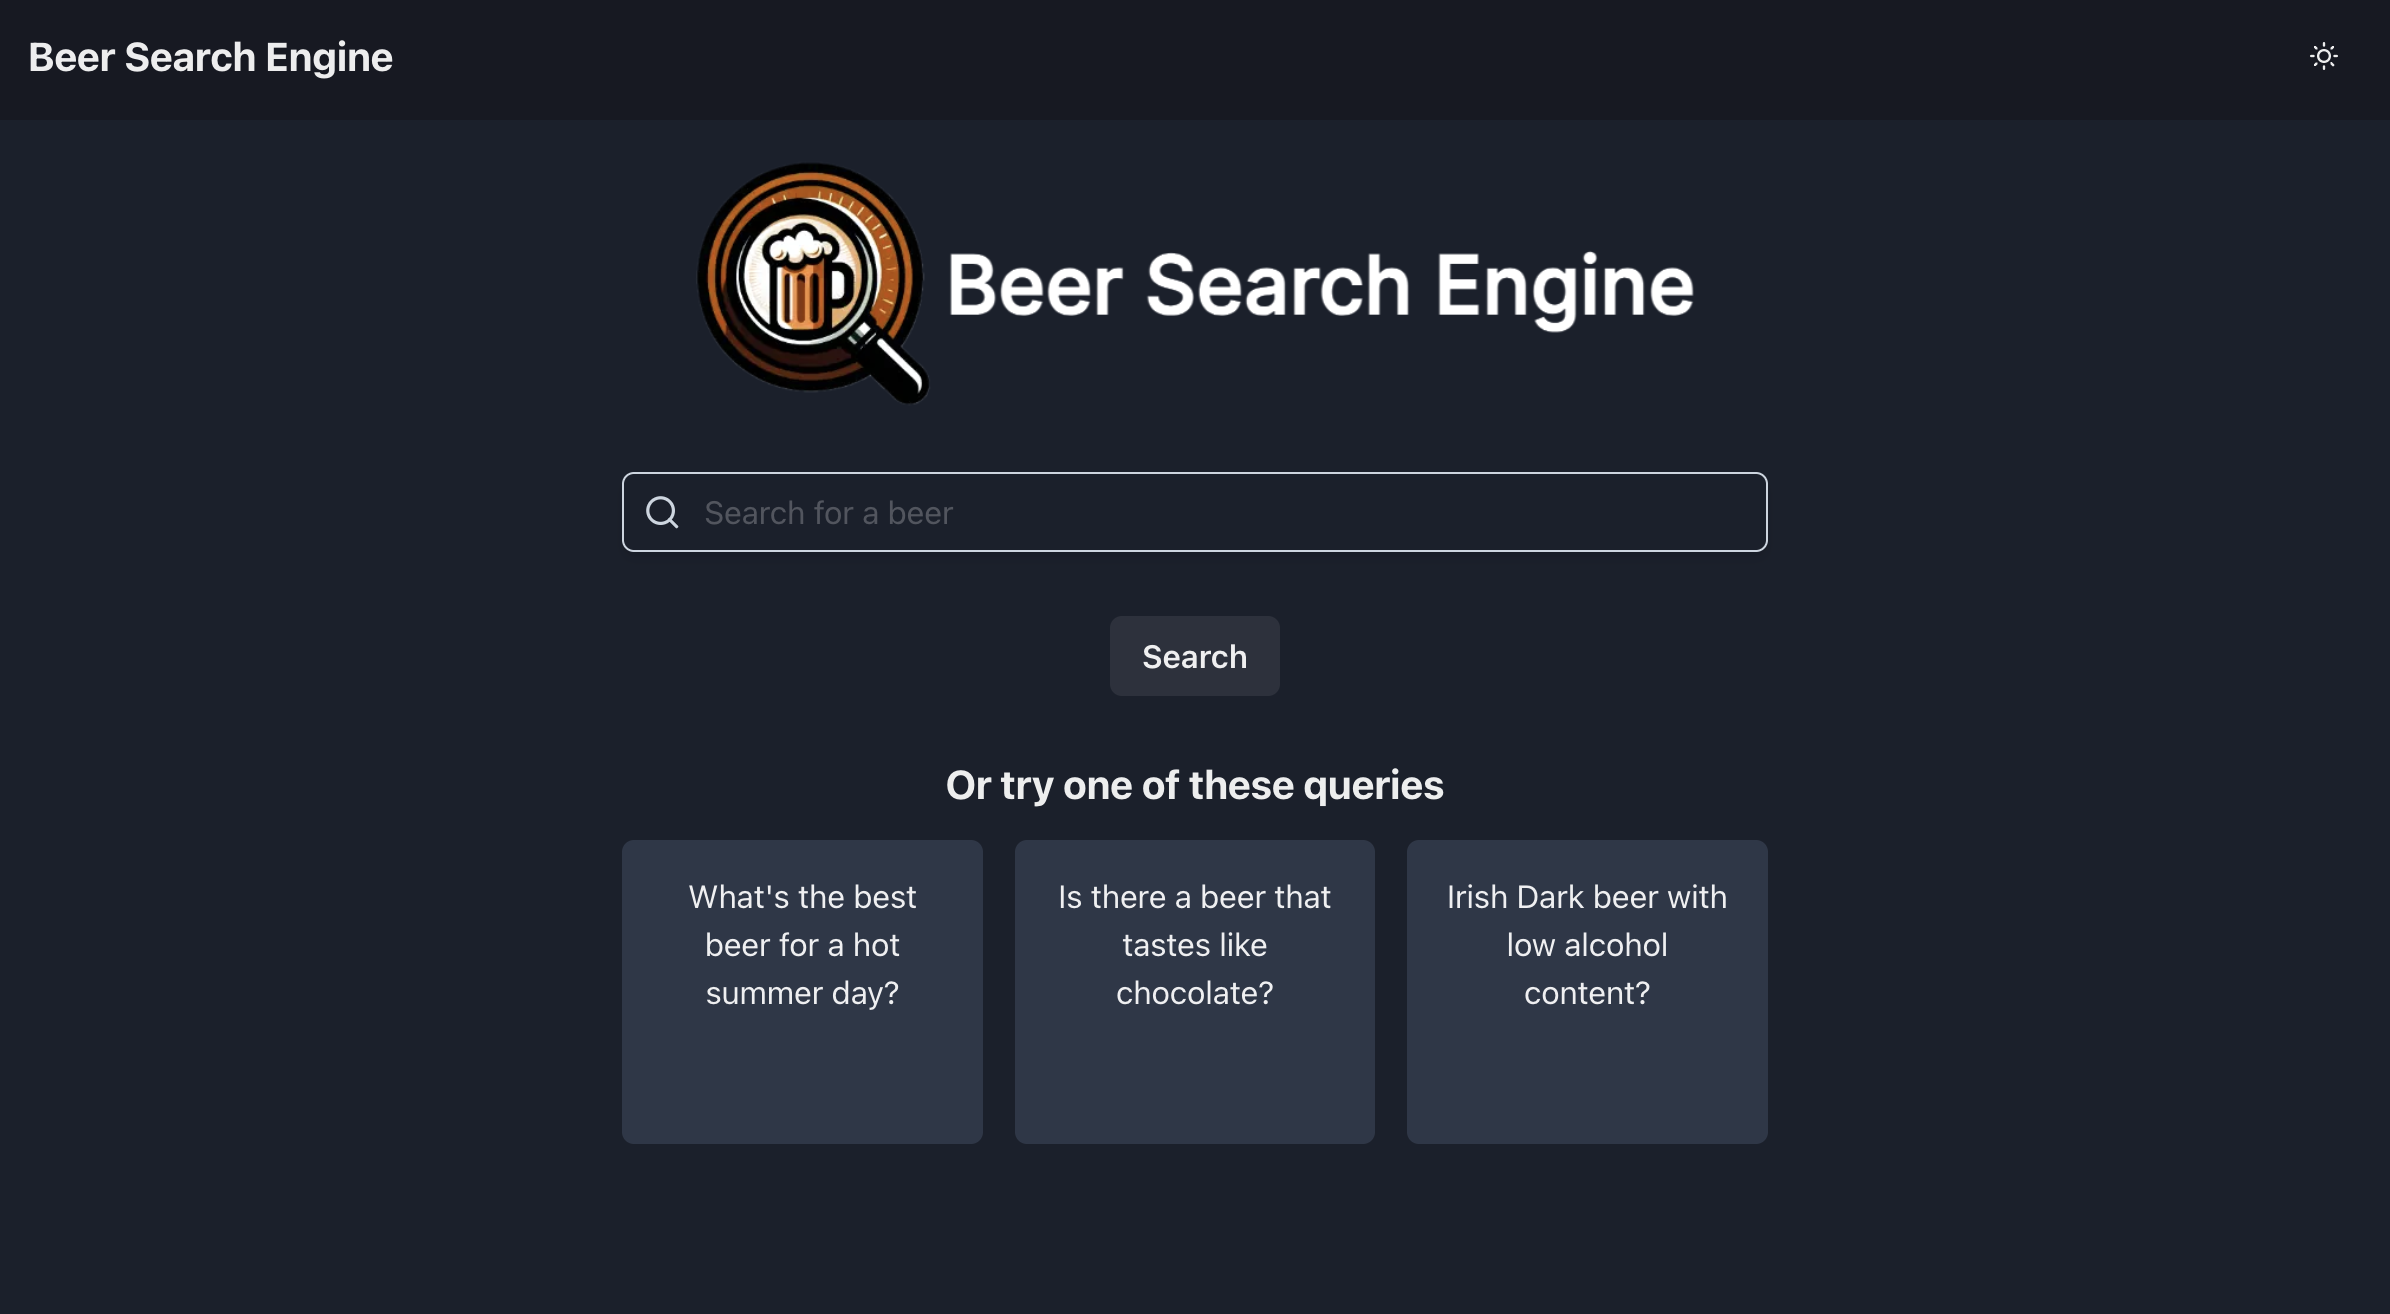
\includegraphics[width=1\textwidth]{img/3_implementation/homepage.png}
  \caption{Web interface homepage that allows the user to perform an initial search.}
  \label{fig:home-page}
\end{figure}

% Search page screenshot
\begin{figure}[H]
  \centering
  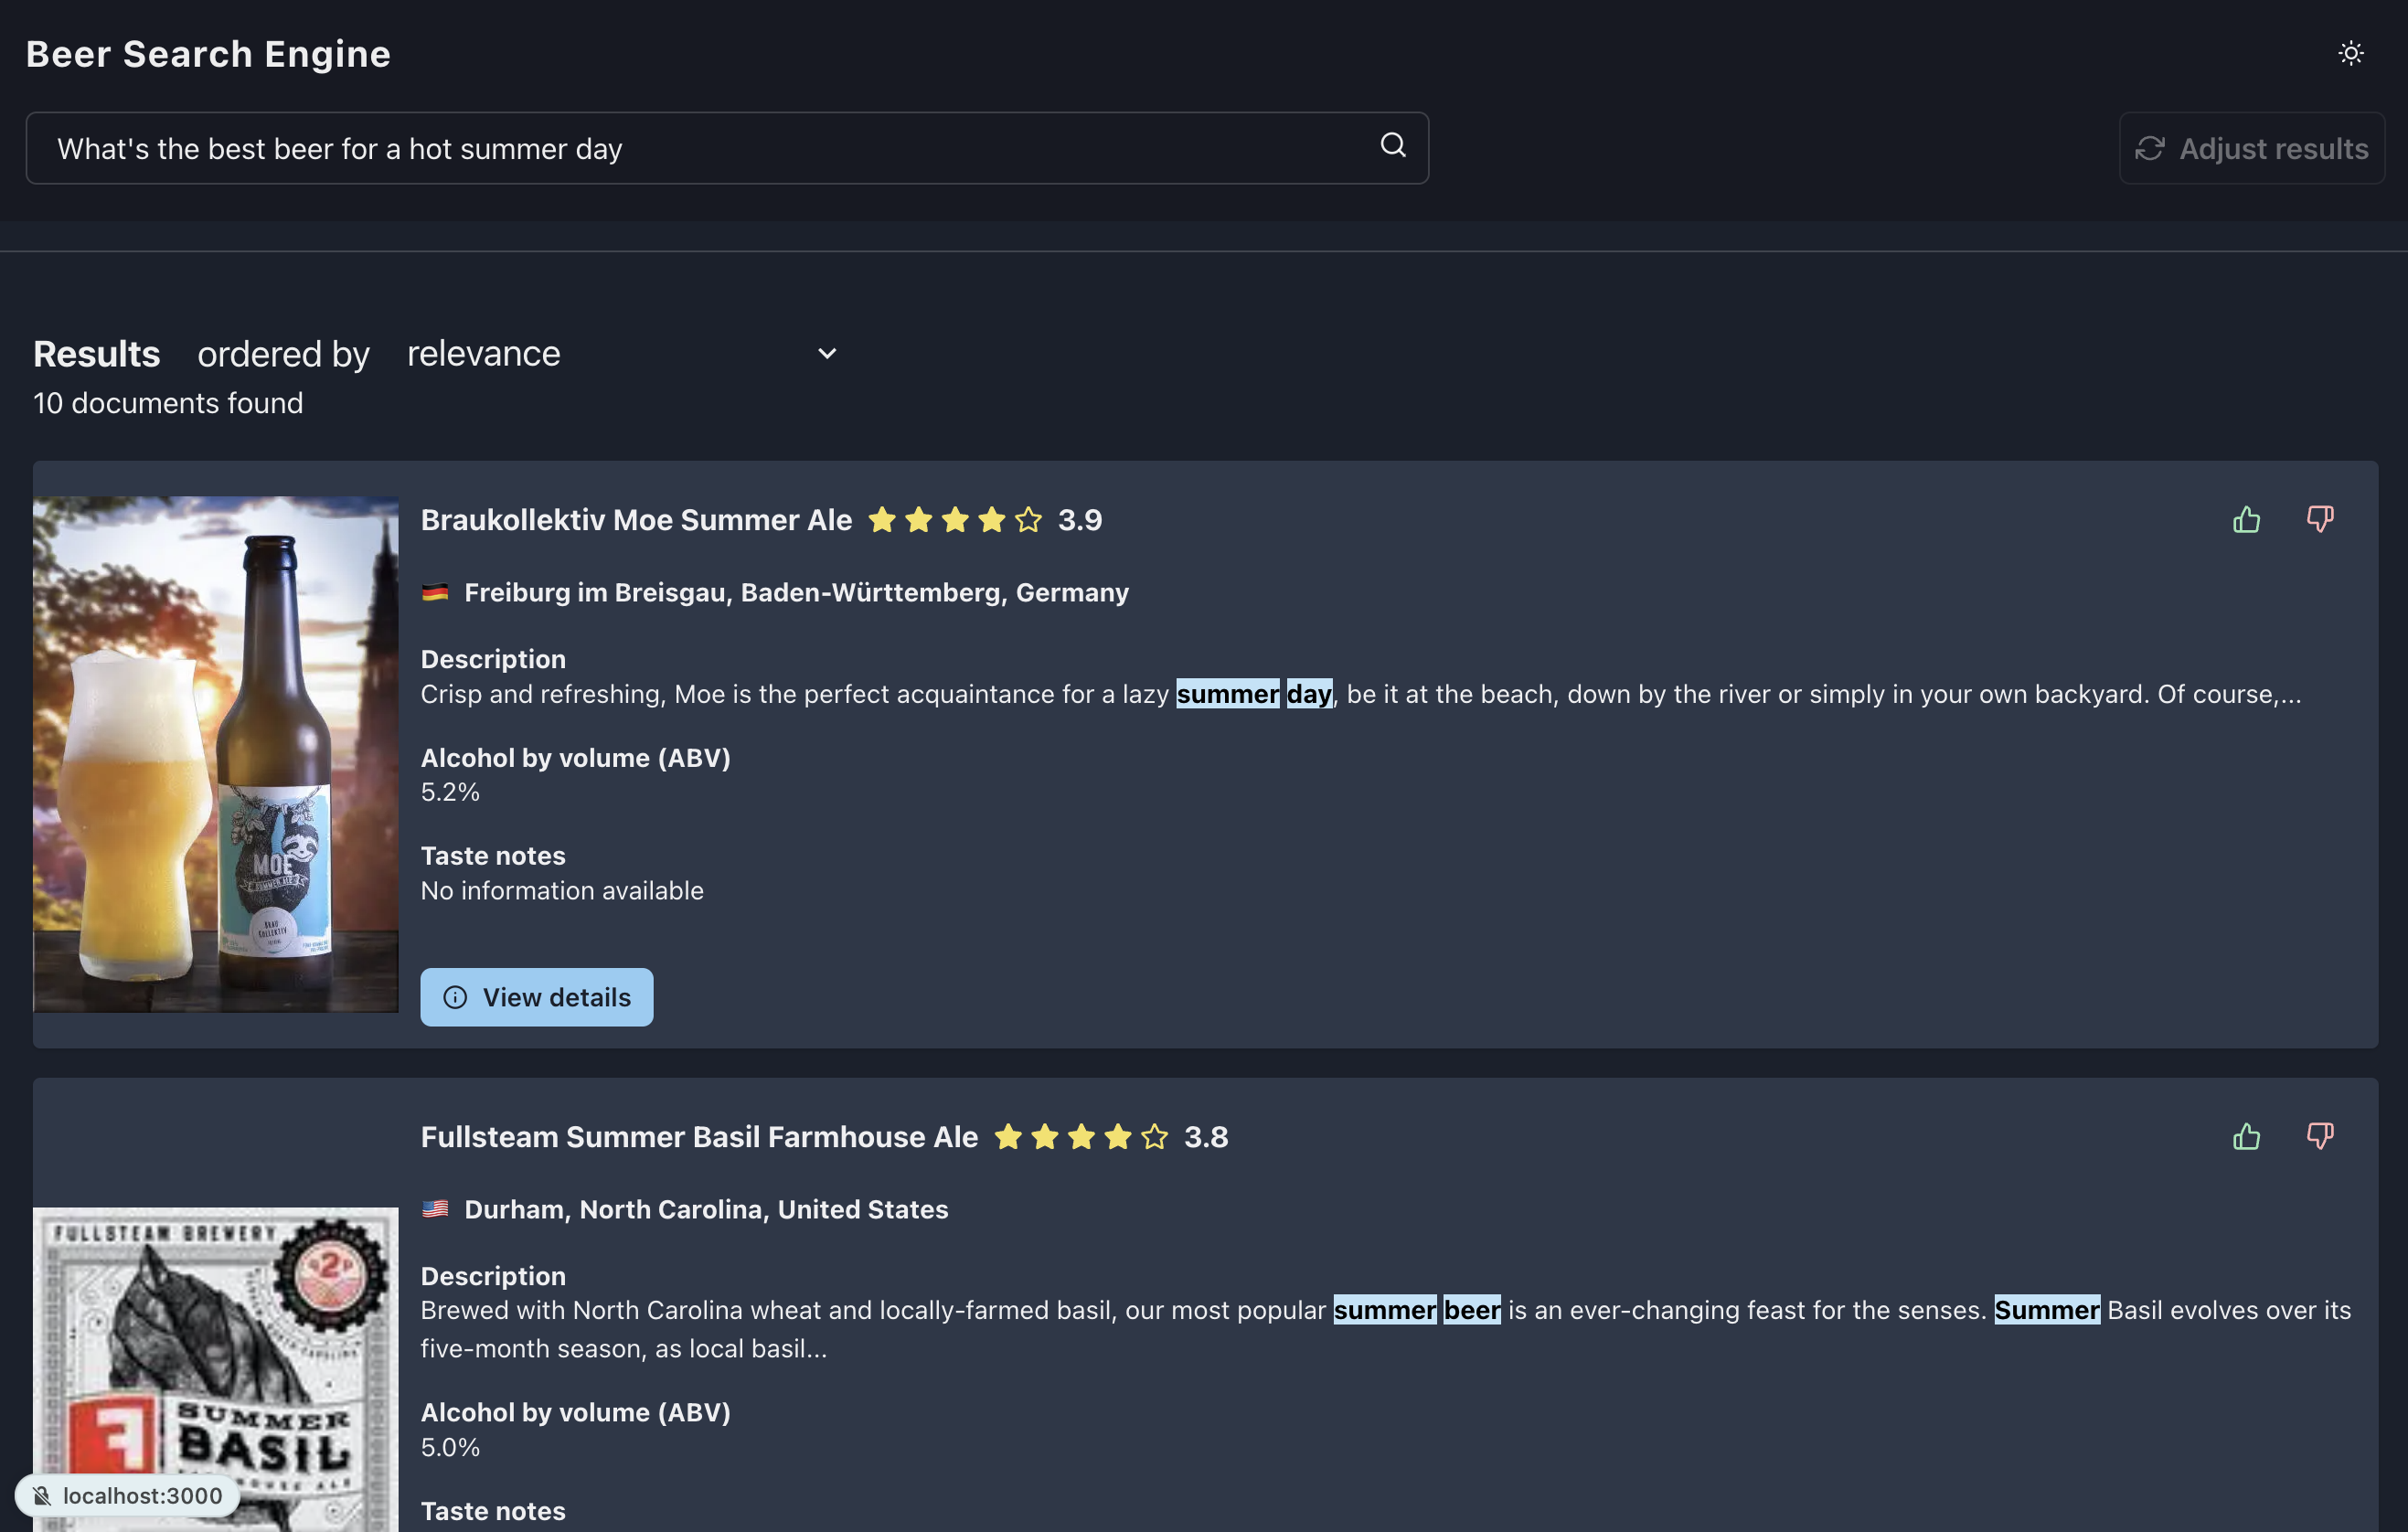
\includegraphics[width=1\textwidth]{img/3_implementation/search-page.png}
  \caption{Search page that allows the user to visualize the query results and perform relevance feedback on them to improve the results.}
  \label{fig:seach-page}
\end{figure}

\subsubsection{Features}

The search engine user interface offers the following features:

\begin{itemize}
  \item Simple and intuitive user interface that allows the user to perform a search in a matter of seconds.
  \item The user can perform relevance feedback to improve the results by explicitly specifying which results are relevant and which are not.
  \item The user can filter the results by multiple criteria: relevance (default), ABV (Alcohol By Volume), rating and name, allowing also to sort the results by ascending or descending order.
  \item Result snippets are provided to give the user a better understanding of why a result is relevant to the query by highlighting the present query terms.
  \item The entire interface supports both light and dark mode to provide a better user experience.
  \item Has been put a strong focus on accessibility, supporting screen readers and choosing colors that are accessible to visually impaired users (refer to Section \ref{sec:lighthouse-benchmark} for more details).
\end{itemize}

\subsubsection{Lighthouse benchmark}
\label{sec:lighthouse-benchmark}

To assess the quality of the frontend, a Lighthouse benchmark has been performed. Lighthouse is an open-source tool that allows to measure the performance, accessibility, best practices and SEO of a web application. The benchmark, focusing on the search page, has been performed on a \textit{MacBook Pro 16" 2023} with the following specifications:

\begin{itemize}
  \item \textbf{CPU}: Apple M2 Pro
  \item \textbf{RAM}: 16 GB
  \item \textbf{OS}: macOS Sonoma 14.0
\end{itemize}

In the following figure (Figure \ref{fig:lighthouse-benchmark}) is possible to see a partial screenshot of the benchmark results.

% Lighthouse benchmark
\begin{figure}[H]
  \centering
  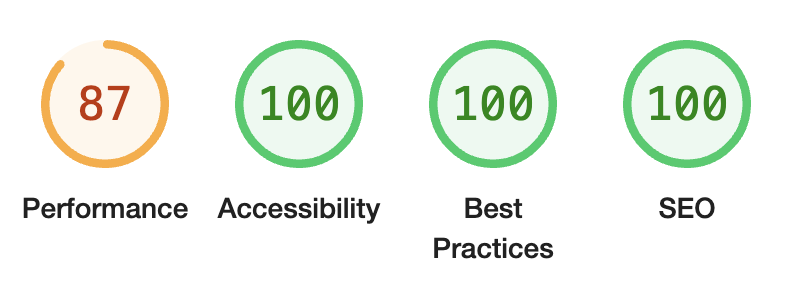
\includegraphics[width=.5\textwidth]{img/3_implementation/lighthouse-benchmark.png}
  \caption{Lighthouse benchmark of the search page of the frontend.}
  \label{fig:lighthouse-benchmark}
\end{figure}

From the results, it is possible to see that the frontend has a perfect score in three of the four categories: accessibility, best practices and \textit{SEO} (Search-Engine Optimization). Performance is the only area not scoring perfectly, mainly due to slow-loading image CDNs.

Slow-loading images are a common problem in web applications, and special measures have been taken to mitigate this issue: images are loaded asynchronously, and a placeholder is shown while the image is loading, allowing the user to browse the results without waiting for the images to load.

\newpage
\subsection{Flow of execution}

To allow readers to better understand the flow of execution of the system, Figure \ref{fig:flow-diagram} outlines how the system handles a user query and how it performs relevance feedback.

% Flow diagram of the system
\begin{figure}[H]
  \centering
  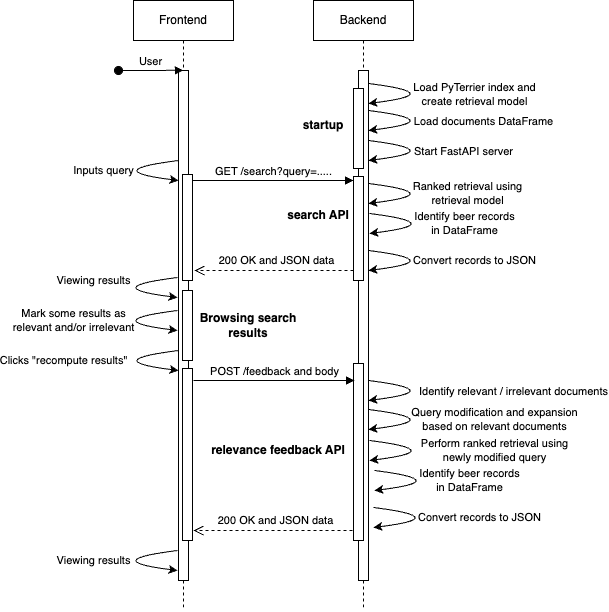
\includegraphics[width=1\textwidth]{img/3_implementation/search-flow.png}
  \caption{Flow diagram describing the execution of the system when a user performs a search and relevance feedback.}
  \label{fig:flow-diagram}
\end{figure}
\newpage
